\section{Inicialização de Máquinas Virtuais}

Por definição, uma máquina virtual é composta por uma \textit{Thread} vinculada a uma \textit{VirtualCPU}.
O fluxo inicia com uma \textit{Thread} comum do sistema que, ao instanciar a máquina virtual, cria sua respectiva \textit{VirtualCPU}.
A partir desse momento, a estrutura de virtualização fica atrelada a essa \textit{Thread}.

\subsection{\textit{GenericVirtualMachine}}

A classe \textit{GenericVirtualMachine} implementa a interface \textit{VirtualMachine} com o objetivo de simplificar a criação de
máquinas virtuais e de seus periféricos. Estruturada como um \textit{template} variádico, ela aceita um número arbitrário de
argumentos para instanciar, mapear e inicializar dinamicamente os dispositivos internos da máquina.

Como parâmetro fundamental, a classe recebe um \textit{Chunk} de memória que delimita a região livre para a execução da máquina virtual.
Todo o restante do espaço de endereçamento do sistema permanece protegido; consequentemente, qualquer acesso a uma região não autorizada
— que não esteja explicitamente mapeada para \gls{mmio} — resultará em uma exceção ou erro crítico.

Nesta modelagem, controladores de interrupção também são tratados como dispositivos,
devendo ser fornecidos explicitamente como parâmetros do \textit{template}, de modo a permitir sua integração ao sistema de eventos
da máquina virtual desde o momento da inicialização.

O processo de inicialização de uma \textit{GenericVirtualMachine} segue o seguinte fluxo:

\vspace{1cm}

\begin{figure}[htbp]
	\begin{center}
	    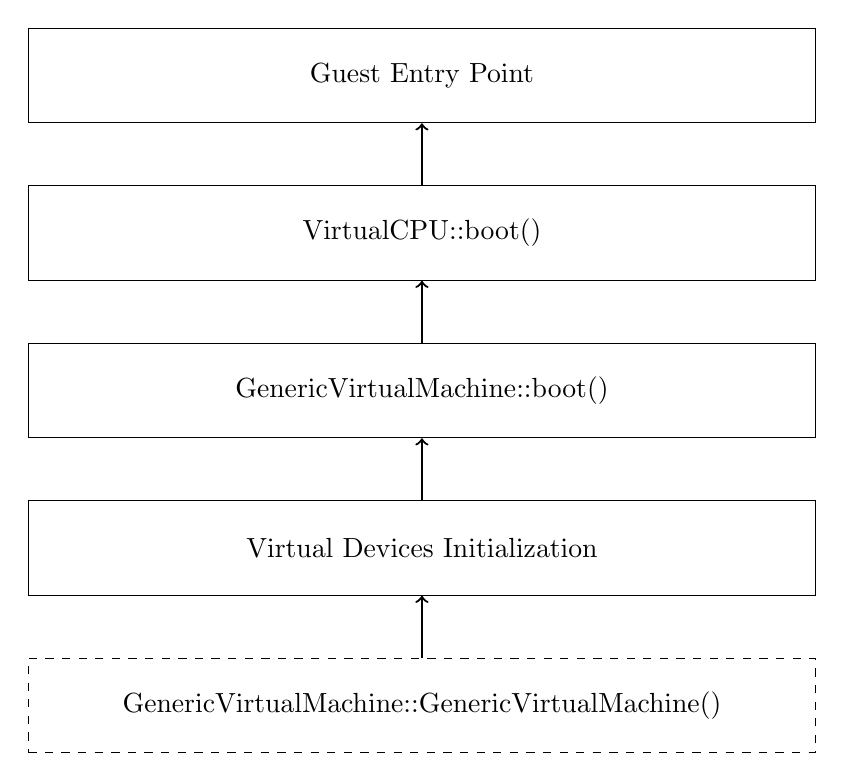
\begin{tikzpicture}
	        \node[rectangle, minimum width=10cm, minimum height=1.2cm, draw, align=center, dashed] (A) at (0,2){GenericVirtualMachine::GenericVirtualMachine()};
	        \node[rectangle, minimum width=10cm, minimum height=1.2cm, draw, align=center] (B) at (0,4){Virtual Devices Initialization};
	        \node[rectangle, minimum width=10cm, minimum height=1.2cm, draw, align=center] (C) at (0,6){GenericVirtualMachine::boot()};
	        \node[rectangle, minimum width=10cm, minimum height=1.2cm, draw, align=center] (D) at (0,8){VirtualCPU::boot()};
	        \node[rectangle, minimum width=10cm, minimum height=1.2cm, draw, align=center] (E) at (0,10){Guest Entry Point};
	        \draw[->, thick] (A) -- (B);
	        \draw[->, thick] (B) -- (C);
	        \draw[->, thick] (C) -- (D);
	        \draw[->, thick] (D) -- (E);
	    \end{tikzpicture}
	\end{center}
	\caption{Fluxo Geral de Inicialização de uma \textit{GenericVirtualMachine}.}
\end{figure}

\subsection{\textit{VirtualCPU}: RISC-V}

Para RISC-V, o processo de inicialização de uma CPU virtual é relativamente simples e pode ser descrito pelo fluxo apresentado
na figura a seguir:

\vspace{1cm}

\begin{figure}[H]
	\begin{center}
	    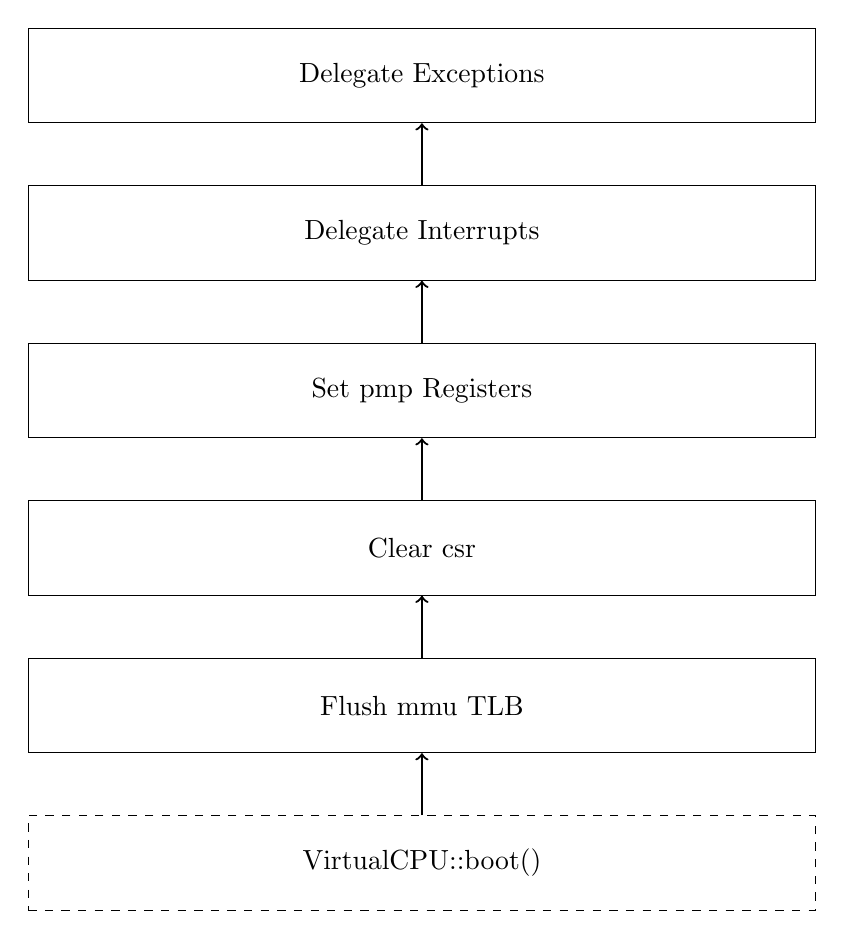
\begin{tikzpicture}
	        \node[rectangle, minimum width=10cm, minimum height=1.2cm, draw, align=center, dashed] (A) at (0,2){VirtualCPU::boot()};
			\node[rectangle, minimum width=10cm, minimum height=1.2cm, draw, align=center] (B) at (0,4){Flush \gls{mmu} TLB};
			\node[rectangle, minimum width=10cm, minimum height=1.2cm, draw, align=center] (C) at (0,6){Clear \glspl{csr}};
			\node[rectangle, minimum width=10cm, minimum height=1.2cm, draw, align=center] (D) at (0,8){Set \gls{pmp} Registers};
	        \node[rectangle, minimum width=10cm, minimum height=1.2cm, draw, align=center] (E) at (0,10){Delegate Interrupts};
	        \node[rectangle, minimum width=10cm, minimum height=1.2cm, draw, align=center] (F) at (0,12){Delegate Exceptions};
	        \draw[->, thick] (A) -- (B);
	        \draw[->, thick] (B) -- (C);
	        \draw[->, thick] (C) -- (D);
	        \draw[->, thick] (D) -- (E);
			\draw[->, thick] (E) -- (F);
	    \end{tikzpicture}
	\end{center}
	\caption{Fluxo Geral de Inicialização de uma \textit{VirtualCPU} RISC-V.}
\end{figure}
